
\section{Introduction}

In Chapter 3, we saw that 
induction can be driven by more than one kind of information,
as perceptual similarity and conceptual knowledge
came into conflict during reasoning.
\citet{Bright2014a}, in their hybrid theory,
proposed a more subtle distinction in inductive reasoning,
between associative and structured knowledge.
While a number of results show that both kinds of knowledge
can drive inductive reasoning, however,
less is known about how these kinds of knowledge interact.
This is the question I seek to answer in this chapter.

As \citet{Bright2014a} note,
theories of induction can be classed in two ways.
Some theories propose that induction is based on structured knowledge:
the world is organised into coherent categories,
and specific knowledge about these categories,
and the often complex relationships between them,
is used as the basis for inference.
One such theory is \citegap{Osherson1990}{'s} similarity coverage model,
that describes inferences about species of animal
with reference to the taxonomic relationships between them.
More recent accounts have generalised this idea,
casting induction as a process of Bayesian inference
\citep{Griffiths2009,Griffiths2005,Heit1998,Kemp2009}.
At the core of these accounts is the notion that
in category-based induction,
we attempt to use the information given in the premises
(i.e. ``Carrots have disease X'')
to update our beliefs about the distribution of this property
across all categories.
To do so, we must be able to express how various categories are related:
the probability that rabbits have a given disease, given that carrots have it,
depends on the means by which diseases can be transmitted between various species,
in this case, through ecological interactions, such as a food chain.
Similarly, biological properties, such as genes,
are most strongly projected according to 
the distance between species in the taxonomic tree \citep{Heit1998,Osherson1990},
while if we know that certain artefacts are found in one city,
geographical distance is used to decide which other cities are likely to
house them \citep{Kemp2009}.

On the other hand,
a number of theories of inductive inference,
and category-based induction in particular,
rely on simpler, \emph{associative} forms of knowledge.
Similarity, including visual similarity,
discussed in Chapter 3, is one such form of knowledge;
things that are similar
\citep[share many properties, or features, that we know of; see][]{Medin1993}
are likely to also share novel properties.
For instance, on learning about two animals, both of which
live underwater, have scales, and breathe through gills,
we do not need to know what a ``fish'' is
to predict that if one lays eggs, the other likely does as well.
Of course, as discussed in Chapter 3, similarity comes in many forms,
and \citet{Fisher2015} make a useful distinction between
perceptual and representational (i.e. knowledge-based) similarity.
Perceptual similarity is most often proposed
as the basis of induction in children
\citep[][see also Chapter 3]{Sloutsky2010,Sloutsky2008,Sloutsky2007}.
A number of theories of induction in adults,
however, are based on the overlap of features
in our mental representations \citep{Rogers2004,Rogers2008,Sloman1993}
or perceptual input \citep{Sloutsky2008,Sloutsky2004}.
Other associative accounts of induction,
including of inductive generalisation during learning, are based on
what is variously referred to as contiguity, co-occurrence, or thematic relations:
things that are often seen together are more likely 
to share properties than things that are not
\citep{Kruschke1992,Rumelhart1986,Rescorla1972}.

% Also cited:
% Colunga & Smith, 2005;
% French, Mareschal, Mermillod, & Quinn, 2004; Jones & Smith, 2002; Sloutsky, Kloos, &
% Fisher, 2007).
% Smith and DeCoster (2000)

\citet{Bright2014a} argue that neither
structured nor associative accounts of induction alone are complete.
As noted by \citet{Murphy1985},
associative accounts of categorisation and induction
fail to capture some of the flexibility and complexity seen in human reasoning.
In particular, participants have been shown to be
sensitive to property effects when reasoning inductively:
the strength of an argument is dependent
on the kind of property projected
\citep{Heit1994,Shafto2007,Shafto2005}.
Therefore, transmittable properties such as infectious diseases
are thought to be shared by animals that are related ecologically,
such as predators and prey in a food chain,
whereas biological properties such as genes are shared 
only by animals that are close together in their taxonomic tree.
It is difficult to account for such flexibility in a purely associative account
\citep[but see work by][]{Sloutsky2008,Rogers2004}.
Structured models such as the Bayesian accounts discussed above \citep[i.e.][]{Kemp2009},
in contrast, draw on different knowledge structures for different inferences,
and so can capture this flexibility in human reasoning.

At the same time, it seems unlikely that 
structured knowledge alone drives inductive reasoning.
Induction is an ubiquitous phenomena, encompassing any inference that goes
``beyond the information given'' \citep{Bruner1973}.
This ranges from simple perceptual inferences,
to the development and postulation of scientific theories
\citep[see][for a taxonomy of inductive inferences]{Kemp2014}.
Furthermore, inductive reasoning is not exclusive to human adults:
similar inferences, although in simpler domains,
must be made both by children, and throughout the animal kingdom.
Associative theories of induction provide accounts that
make more reasonable claims about the cognitive abilities
required to reason inductively.
Indeed, in the spirit of \citet{Simon1956},
associative processes may \emph{satisfice},
often yielding the same inferences as structured accounts,
but with considerably less effort.

Faced with this dichotomy between associative and structured knowledge in induction,
\citet{Bright2014a} proposed a theory that combines both forms of knowledge.
This \emph{hybrid} theory claims
that both kinds of knowledge are drawn upon during reasoning,
with a key distinction between the two being their processing characteristics.
By this account, associative knowledge can be retrieved quickly and easily,
while structured knowledge is slower to retrieve,
and places greater demands on working memory to utilise.

Evidence for this hybrid theory
comes from experiments that manipulate 
the processing conditions under which participants reason.
This research is discussed in more detail in Chapter 1, but to recapitulate,
participants' inferences (their choices, or ratings of argument strength)
are predicted by measures of associative knowledge under all circumstances.
Furthermore, under favourable conditions only
(i.e. in the absence of time pressure, or cognitive load),
inferences are additionally predicted by
appropriate measures of structured knowledge,
such as whether participants believed two species
belonged to the same taxonomic group
when reasoning about biological properties.

Of particular relevance to this thesis, which focuses on \emph{conflict} in reasoning,
\citeauthor{Bright} (\citeyear{Bright}, see also \citealp[Chapter 5]{Crisp-Bright2010})
report a version of the inductive triad task \citep{Gelman1986}
that places associative and structured knowledge directly in conflict.
In the trial shown in Figure~\ref{fig:crisp_screenshot}, for example,
participants were told a biological property of carrots (they have ``C5s cells''),
and chose between generalising this property to rabbits, or to bamboo.
Carrots and rabbits are strongly associated,
and so a participant relying on associative knowledge
would project a property from carrots to rabbits.
This is despite the fact that the link between the species is a food chain,
and so doesn't provide a means for them to share a biological property.
Carrots and bamboo, on the other hand, are both plants,
and so are more likely to share such a property.
The associative link between the two species, however,
is substantially weaker, and so projecting the property to bamboo
requires that one inhibits the associative knowledge linking carrots and rabbits
before one can draw on the structured link between carrots and bamboo instead.
Consistent with the hybrid theory,
participants were less likely to select the
taxonomically-related response option
over a strongly associated foil in this task
when under heavy cognitive load,
or if they had poor semantic inhibitory control
\citep[a measure of their ability to inhibit
  task-irrelevant semantic information;][]{Markovits2004,Burgess1996a}.
Like most studies that analyse only participants' ultimate responses, however,
while these results do reveal what information drove participants' final choices,
we are limited in what conclusions we can draw about
how different processes interact during this task.
To address this shortcoming, in this chapter I present
a mouse tracking extension of the \citet{Bright} triad task.

\begin{figure}[ht]
  \centering
  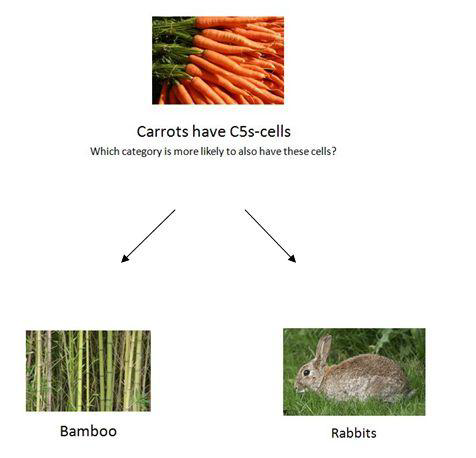
\includegraphics[width=\figurewidth]{imgs/crisp_screenshot.png}
  \caption[A conflict trial from \citet{Bright}.]{
    A conflict trial from \citet{Bright}.
    Participants learn that carrots posses the given biological property,
    and asked which of the other two species, bamboo or rabbits,
    are likely to share this property.
    \label{fig:crisp_screenshot} }
\end{figure}


How might associative and structured knowledge interact during this task?
Again, I propose two possibilities.
First, it may be that people selectively draw on associative knowledge
\emph{or} structured knowledge for a given inference.
In this case, we would expect to find
little evidence of actual conflict during reasoning,
as both kinds of knowledge would not compete during a single trial.
This would lead to cursor trajectories where
participants move directly towards one or other option, and then select it,
rather than changing direction mid-flight.
The second possibility is that
associative knowledge may be activated early in reasoning,
but be later overridden, at least some of the time,
by slowly-retrieved, more cognitively demanding structured knowledge.
In this case, participants would be conflicted
when they do override, or at least attempt to override,
their association-driven response.
Cursor trajectories in this case should largely be
initially drawn to the foil species
when it is cued by associative knowledge,
but also likely to override this initial movement
and select the correct species instead
at least some of the time.



